\documentclass{article}

%other packages
\usepackage[a4paper]{geometry}
\usepackage{longtable}
\usepackage{wrapfig}
\setlength\parindent{0pt}
\usepackage{enumitem}
\usepackage[table]{xcolor}
\usepackage{polynom}
\def\scaleint#1{\vcenter{\hbox{\scaleto[3ex]{\displaystyle\int}{#1}}}}
\usepackage{array}
\newcolumntype{C}{>{{}}c<{{}}} % for '+' and '-' symbols
\newcolumntype{R}{>{\displaystyle}r} % automatic display-style math mode 
\usepackage{tabularray}
\usepackage{dcolumn,tabularx,booktabs}

%maths
\usepackage{mathtools}
\usepackage{amsmath}
\usepackage{amssymb}
\usepackage{amsfonts}
\usepackage{autobreak}

%tikzpicture
\usepackage{tikz}
\usepackage{scalerel}
\usepackage{pict2e}
\usepackage{tkz-euclide}
\usepackage{tikz-3dplot}
\usetikzlibrary{calc}
\usetikzlibrary{patterns,arrows.meta}
\usetikzlibrary{shadows}
\usetikzlibrary{external}

%pgfplots
\usepackage{pgfplots}
\pgfplotsset{compat=newest}
\usepgfplotslibrary{statistics}
\usepgfplotslibrary{fillbetween}

\pgfplotsset{
    standard/.style={
    axis line style = thick,
    trig format=deg,
    enlargelimits,
    axis x line=middle,
    axis y line=middle,
    enlarge x limits=0.15,
    enlarge y limits=0.15,
    every axis x label/.style={at={(current axis.right of origin)},anchor=north west},
    every axis y label/.style={at={(current axis.above origin)},anchor=south east}
    },
    width=.96\linewidth,
    height=2.5cm,
    scale only axis=true
}

\begin{document}

{\bf{}ANGLES}
\hrule

\vspace{10pt}

Angles can be measured in radians or degrees. A complete revolution is $360^\circ$ or $2\pi\textnormal{rad}$.

\begin{center}
\bgroup
\def\arraystretch{1.5}
\begin{tabular}{|l|}
\hline
$\pi\textnormal{rad}=180^\circ$\\
\hline
\end{tabular}
\egroup
\end{center}

For a circular sector with central angle $\theta$ and radius $r$ subtending an arc with lenth $a$, \fbox{$\theta=\frac{a}{r}$}

\vspace{10pt}

{\bf{}THE TRIGONOMETRIC FUNCTIONS}
\hrule

\vspace{10pt}

The opposite and adjacent sidelengths of a $\frac{1}{4}\pi$ right triangle are of equal value.

\vspace{10pt}

The opposite and adjacent sidelengths of a $\frac{1}{3}\pi$ or $\frac{1}{6}\pi$ right triangle can be found by completing the equilateral triangle to solve for one and then using the pythagorean theorem to solve for the other.

\vspace{10pt}

{\bf{}TRIGONOMETRIC IDENTITIES}
\hrule

\vspace{10pt}

It follows from the pythagorean theorem that \fbox{$\sin^2\theta+\cos^2\theta=1$}

\vspace{10pt}

We can multiple and divide both sides by squared trig functions to obtain more identities.

The sine function is odd and the cosine function is even.

The {\bf{}addition} formulas are proven in Ex.85-87.

\bgroup
\def\arraystretch{1.5}
\[\boxed{\begin{aligned}
\sin(x+y)&=\sin x\cos y+\cos x\sin y\\
\cos(x+y)&=\cos x\cos y-\sin x\sin y
\end{aligned}}\]
\egroup

By substituting $-y$ for $y$, we obtain the subtraction formulas.

\bgroup
\def\arraystretch{1.5}
\[\boxed{\begin{aligned}
\sin(x-y)&=\sin x\cos y-\cos x\sin y\\
\cos(x-y)&=\cos x\cos y+\sin x\sin y
\end{aligned}}\]
\egroup

Then, by dividing the addition and subtraction formulas, we obtain the corresponding formulas for tangent.

\bgroup
\def\arraystretch{1.5}
\[\boxed{\begin{aligned}
\tan(x+y)&=\frac{\tan x+\tan y}{1-\tan x\tan y}\\
\tan(x-y)&=\frac{\tan x-\tan y}{1+\tan x\tan y}
\end{aligned}}\]
\egroup

If we put $y=x$ in the addition formulas, we get the {\bf{}double-angle formulas}.

\bgroup
\def\arraystretch{1.5}
\[\boxed{\begin{aligned}
\cos\sin2x&=2\sin x\cos x\\
\cos2x&=\cos^2x-\sin^2x
\end{aligned}}\]
\egroup

Then by using the pythagorean identity, we can obtain alternate forms of $\cos2x$.

\bgroup
\def\arraystretch{1.5}
\[\boxed{\begin{aligned}
\cos2x&=2\cos^2x-1\\
&=1-2\sin^2x
\end{aligned}}\]
\egroup

If we now solve these equations for $\sin^2x$ and $\cos^2x$, we get the {\bf{}half-angle formulas}.

\bgroup
\def\arraystretch{1.5}
\[\boxed{\begin{aligned}
\cos^2x&=\frac{1+\cos2x}{2}\\
\sin^2x&=\frac{1-\cos2x}{2}
\end{aligned}}\]
\egroup

The {\bf{}product rules} can be deduced from the addition and subtraction formulas.

\bgroup
\def\arraystretch{1.5}
\[\boxed{\begin{aligned}
\sin x\cos y&=\frac{1}{2}[\sin(x+y)+\sin(x-y)]\\
\cos x\cos y&=\frac{1}{2}[\cos(x+y)+\cos(x-y)]\\
\sin x\sin y&=\frac{1}{2}[\cos(x-y)-\cos(x+y)]
\end{aligned}}\]
\egroup

{\bf{}EXAMPLE} Find all values of $x$ in the interval $[0,2\pi]$ such that $\sin x=\sin2x$.

\vspace{10pt}

Using the double angle formula, we rewrite the given equation as

\[\sin x=2\sin x\cos x\qquad\textnormal{or}\qquad\sin x(1-2\cos x)=0\]

Therefore there are two possibilities:

\[\begin{aligned}[t]
\sin x&=0\\
x&=0,\pi,2\pi
\end{aligned}
\qquad\textnormal{or}\qquad
\begin{aligned}[t]
1-2\cos x&=0\\
\cos x&=\frac{\pi}{3},\frac{5\pi}{3}
\end{aligned}\]

The given equation has five solutions: $0,\ \pi/3,\ \pi,\ 5\pi/3,\ \textnormal{and}\ 2\pi$

\begin{center}
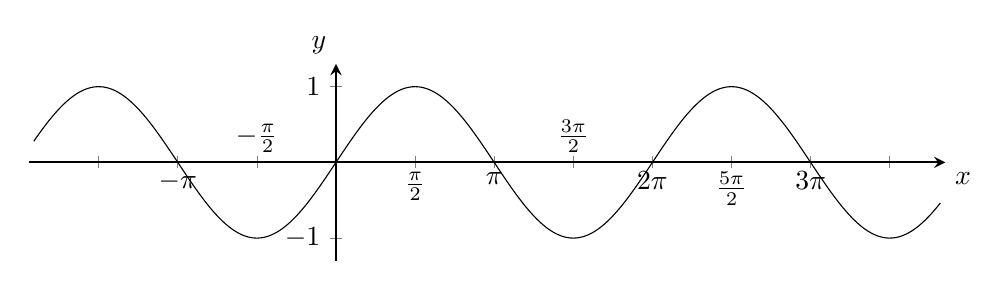
\begin{tikzpicture}
\begin{axis}[
standard,
xmin=-4, xmax=10,
xtick={-3.14159*3/2,-3.14159,-3.14159/2,3.14159/2,3.14159,3.14159*3/2,3.14159*2,3.14159*5/2,3.14159*3,3.14159*7/2}, ytick={-1,1},
xticklabels={}, yticklabels={$-1$,$1$},
xlabel={$x$}, ylabel={$y$},]
\addplot[domain=-6:12,samples=300] {sin(deg(x))};
\node[below] at (-3.14159,0) {$-\pi$};
\node[below] at (3.14159,0) {$\pi$};
\node[below] at (3.14159*3,0) {$3\pi$};
\node[above] at (-3.14159/2,0) {$-\frac{\pi}{2}$};
\node[below] at (3.14159/2,0) {$\frac{\pi}{2}$};
\node[above] at (3.14159*3/2,0) {$\frac{3\pi}{2}$};
\node[below] at (3.14159*2,0) {$2\pi$};
\node[below] at (3.14159*5/2,0) {$\frac{5\pi}{2}$};
\end{axis}
\end{tikzpicture}
\end{center}

\begin{center}
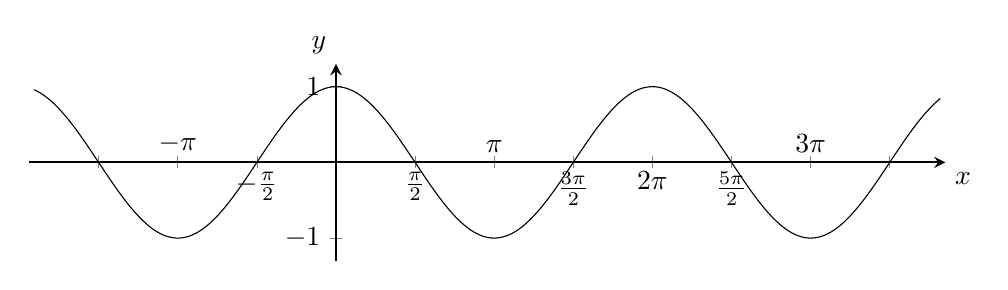
\begin{tikzpicture}
\begin{axis}[
standard,
xmin=-4, xmax=10,
xtick={-3.14159*3/2,-3.14159,-3.14159/2,3.14159/2,3.14159,3.14159*3/2,3.14159*2,3.14159*5/2,3.14159*3,3.14159*7/2}, ytick={-1,1},
xticklabels={}, yticklabels={$-1$,$1$},
xlabel={$x$}, ylabel={$y$},]
\addplot[domain=-6:12,samples=300] {cos(deg(x))};
\node[above] at (-3.14159,0) {$-\pi$};
\node[above] at (3.14159,0) {$\pi$};
\node[above] at (3.14159*3,0) {$3\pi$};
\node[below] at (-3.14159/2,0) {$-\frac{\pi}{2}$};
\node[below] at (3.14159/2,0) {$\frac{\pi}{2}$};
\node[below] at (3.14159*3/2,0) {$\frac{3\pi}{2}$};
\node[below] at (3.14159*2,0) {$2\pi$};
\node[below] at (3.14159*5/2,0) {$\frac{5\pi}{2}$};
\end{axis}
\end{tikzpicture}
\end{center}


\end{document}